% #######################################
% ########### FILL THESE IN #############
% #######################################
\def\mytitle{Verifying the Given Expression using Boolean Laws}
\def\mykeywords{}
\def\myauthor{Aluru Ajay}
\def\contact{19pa1a0410@vishnu.edi.in}
\def\mymodule{Future Wireless Communication-(FWC22029)}
% #######################################
% #### YOU DON'T NEED TO TOUCH BELOW ####
% #######################################
\documentclass[10pt, a4paper]{article}
\usepackage[a4paper,outer=1.5cm,inner=1.5cm,top=1.75cm,bottom=1.5cm]{geometry}
\twocolumn
\usepackage{graphicx}
\graphicspath{{./images/}}
%colour our links, remove weird boxes
\usepackage[colorlinks,linkcolor={black},citecolor={blue!80!black},urlcolor={blue!80!black}]{hyperref}
%Stop indentation on new paragraphs
\usepackage[parfill]{parskip}
%% Arial-like font
\usepackage{lmodern}
\renewcommand*\familydefault{\sfdefault}
%Napier logo top right
\usepackage{watermark}
%Lorem Ipusm dolor please don't leave any in you final report ;)
\usepackage{lipsum}
\usepackage{xcolor}
\usepackage{listings}
%give us the Capital H that we all know and love
\usepackage{float}
%tone down the line spacing after section titles
\usepackage{titlesec}
%Cool maths printing
\usepackage{amsmath}
%PseudoCode
\usepackage{algorithm2e}

\titlespacing{\subsection}{0pt}{\parskip}{-3pt}
\titlespacing{\subsubsection}{0pt}{\parskip}{-\parskip}
\titlespacing{\paragraph}{0pt}{\parskip}{\parskip}
\newcommand{\figuremacro}[5]{
    \begin{figure}[#1]
        \centering
        \includegraphics[width=#5\columnwidth]{#2}
        \caption[#3]{\textbf{#3}#4}
        \label{fig:#2}
    \end{figure}
}

\lstset{
  escapeinside={/@}{@/}, language=C++,
  basicstyle=\fontsize{8.5}{12}\selectfont,
  numbers=left,numbersep=2pt,xleftmargin=2pt,frame=tb,
    columns=fullflexible,showstringspaces=false,tabsize=4,
    keepspaces=true,showtabs=false,showspaces=false,
    backgroundcolor=\color{white}, morekeywords={inline,public,
    class,private,protected,struct},captionpos=t,lineskip=-0.4em,
  aboveskip=10pt, extendedchars=true, breaklines=true,
  prebreak = \raisebox{0ex}[0ex][0ex]{\ensuremath{\hookleftarrow}},
  keywordstyle=\color[rgb]{0,0,1},
  commentstyle=\color[rgb]{0.133,0.545,0.133},
  stringstyle=\color[rgb]{0.627,0.126,0.941}
}

\thiswatermark{\centering \put(0,-90.0){
\includegraphics[scale=0.05]{iith.jpg}} }
\title{\mytitle}
\author{\myauthor\hspace{1em}\\\contact\\IITH\hspace{0.5em}-\hspace{0.5em}\mymodule}
\date{}
\hypersetup{pdfauthor=\myauthor,pdftitle=\mytitle,pdfkeywords=\mykeywords}
\sloppy
% #######################################
% ########### START FROM HERE ###########
% #######################################
\begin{document}
  \maketitle
\tableofcontents


\section{ABSTRACT}

The objective of this manual is to show how to Verify the
Boolean Expression U' + V = U'V' + U'.V+U.V
\section{INTRODUCTION}

Boolean algebra problems can be solved using these Boolean algebra laws.There are few boolean algebra rules to be followed while solving problems.In order to define the functioning of a digital logic circuit, Boolean Algebra makes use of a set of Laws and Rules.Along with being used to represent digital input and output, the logic symbols “0” and “1” may also be used as constants to indicate a circuit or contact that is either permanently “Open” or “Closed.”



\section{MATHEMATICAL PROOF}

To prove: U' + V = U'V' + U'.V+U.V

  $ RHS	=UV+UV+UV $
    \\   = U'.(V+V') + U.V    (using distributive law)
    \\    =U'.(1) + U.V	 (using complement law)
	  \\  =U'+U.V		    (using identity law)
	   \\ =(U'+U). (U'+V)	(using distributive law)
	   \\ =1.(U'+V)		(using complement law)
	    \\=U'+V			(using identity law)\\
 RHS	= LHS       

\section{COMPONENTS}
\begin{figure}[h]
    \centering
    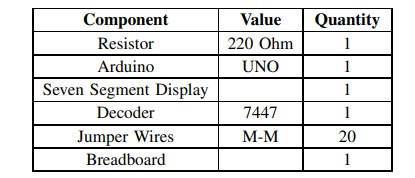
\includegraphics[width=0.4\textwidth]{Components.jpg}
    \caption{list of components}
    \label{fig:my_label}
     \end{figure}
\newpage
\section{HARDWARE}
Problem 5.1. Make connections between the seven segment display  and the 7447 IC
\\Problem 5.2. Make connections to the lower pins of the 7447  and connect VCC = 5V. You should see the number 0 displayed for 0000and 1 for 0001.


\begin{figure}[h]
    \centering
    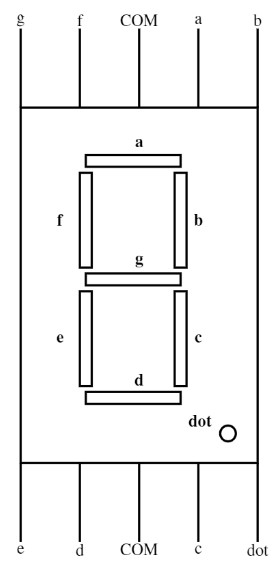
\includegraphics[width=0.2\textwidth]{7segpo.jpg}
    \caption{seven segment}
    \label{fig:my_label}
\end{figure}


\begin{figure}[h]
    \centering
    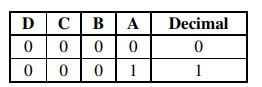
\includegraphics{decimal.jpg}
    \caption{}
   % \laProblem 
\end{figure}  
  
Problem 4.3. Complete Table 2.2 by generating all
numbers between 0-9
\section{SOFTWARE}

1. Connect the Arduino to the computer.
\\2. Download the following directory
\\subsection{Code Link} 
\vspace{5mm} 
\begin{lstlisting} 
\\GITHUB : https://github.com/19PA1AO410/FWC-Module-1/blob/main/Code-FWC.txt
\end{lstlisting} 

\section{CONCLUSION}
Lets consider the the both(LHS and RHS) equations as A and B
\\CASE 1: If A=B,then seven segment shows "1"
\\CASE 2: If A!=B,then seven segment shows"0"




\end{document}